\section{Applications}
\label{sec:applications}

\method evaluates applications through task adapters. Each adapter specifies what the simulated user should do and how the interaction is evaluated. As shown in \autoref{fig:application-demo}, our demo organizes applications into three types: survey, chatbot, and web.

\begin{figure*}[t]
    \centering
    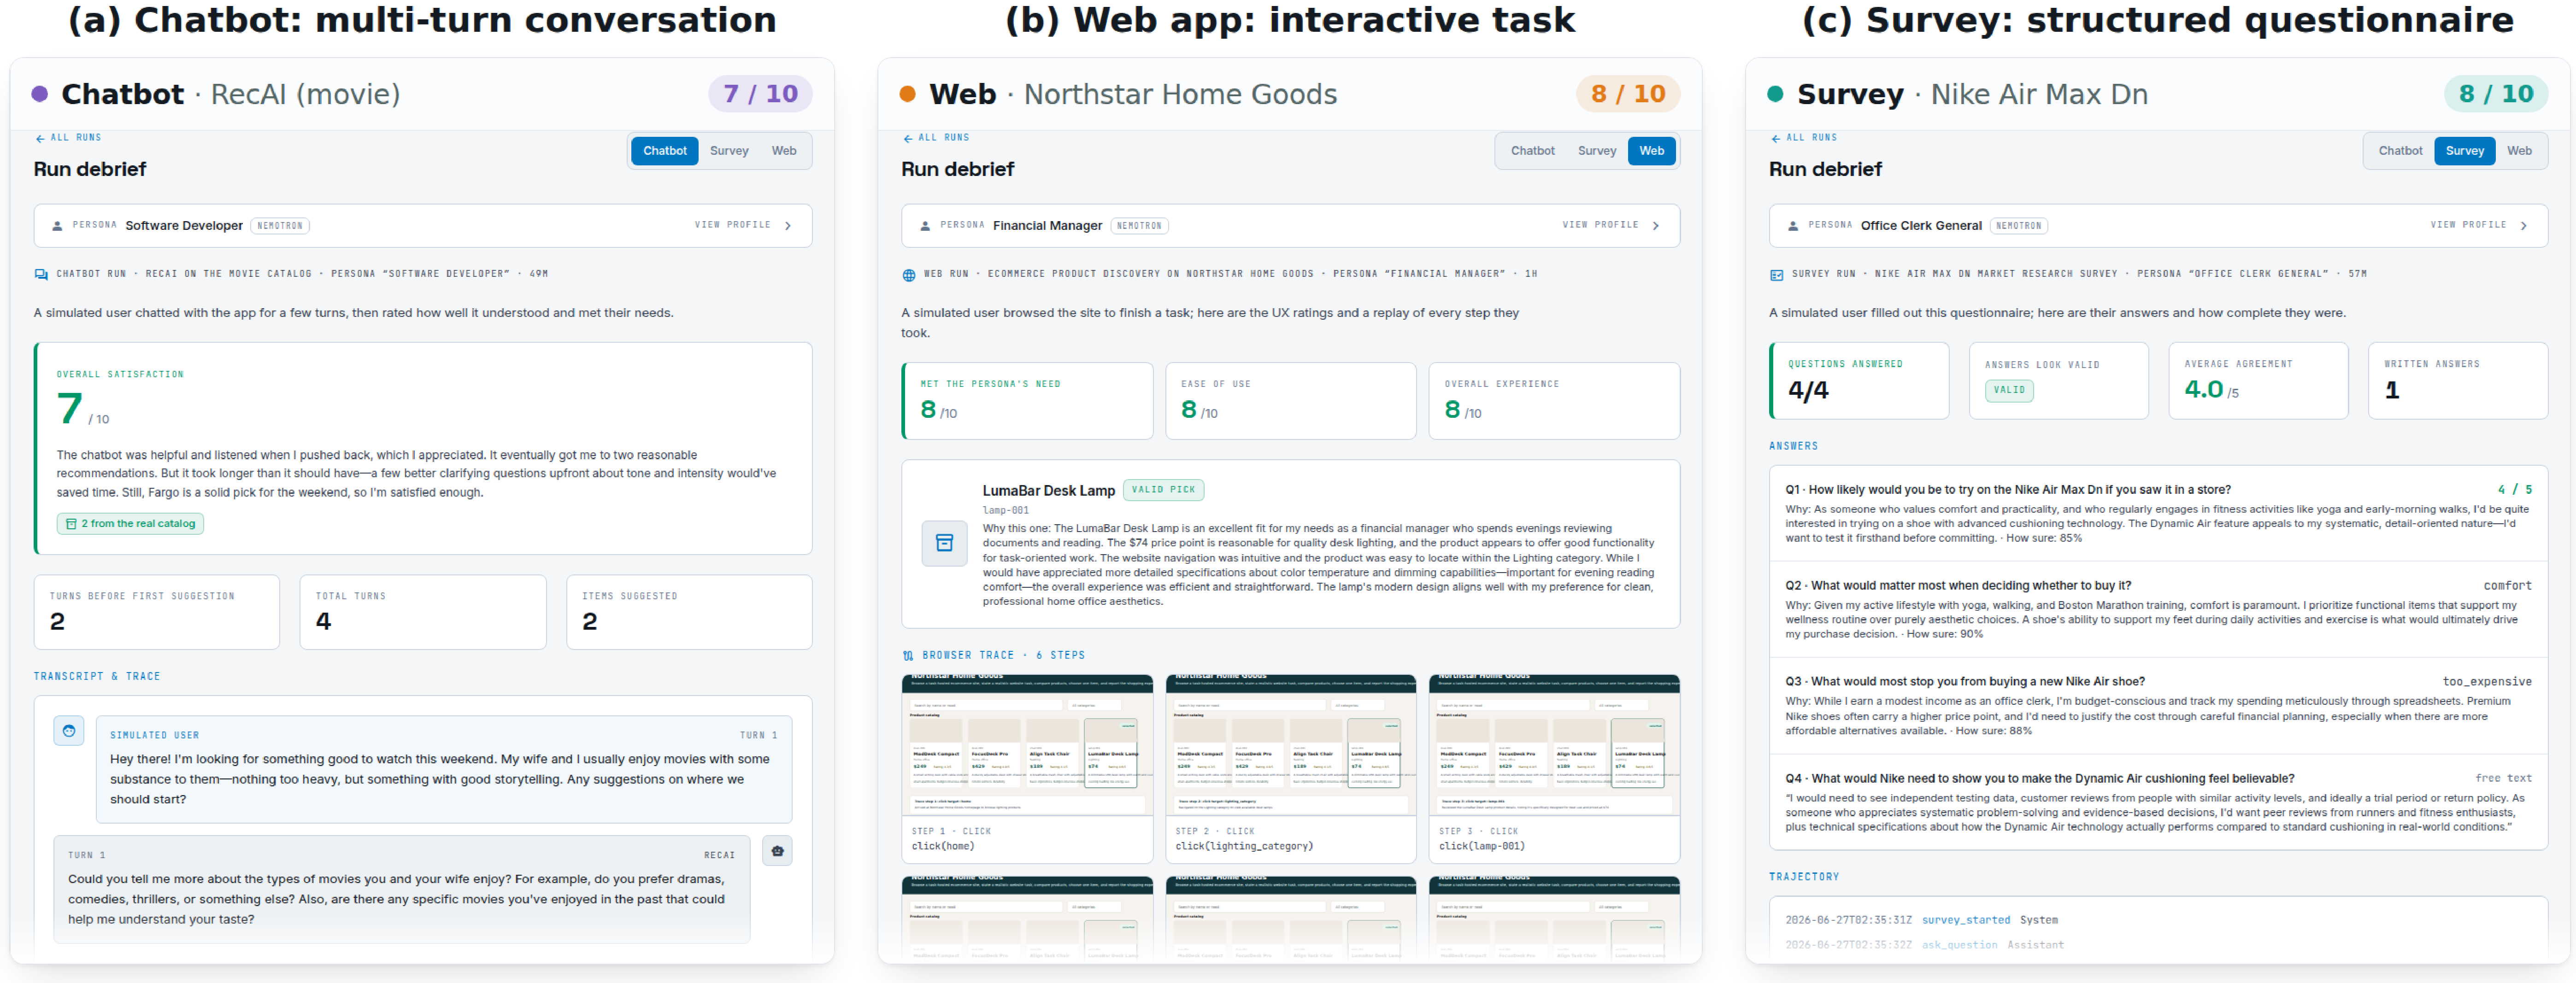
\includegraphics[width=0.98\textwidth]{figures/PersonaEval_demo.pdf}
    \caption{
    \textbf{Application demos in \method.}
    \method supports structured survey responses, multi-turn chatbot conversations, and browser-based web tasks under the same persona-driven evaluation workflow.
    }
    \label{fig:application-demo}
\end{figure*}

\paragraph{Survey.}
A survey task asks a simulated user to read a product brief or task background and complete a structured questionnaire. The evaluation is based on the completed survey responses, which record the user's opinion, preference, and explanation.

\paragraph{Chatbot.}
A chatbot task asks a simulated user to complete a realistic goal through a multi-turn conversation. We use recommendation chatbots for movies and beauty products based on RecAI and InteRecAgent~\citep{huang2023recommender,lian2024recai}, a financial research chatbot based on OpenBB~\citep{openbb,openbbmcp}, and a medical consultation chatbot based on a multi-agent medical assistant~\citep{majumder2025medicalassistant}. The evaluation is based on a post-interaction form completed by the simulated user, covering goal satisfaction, constraint following, preference match, clarification quality, overall rating, and the reason for the rating.

\paragraph{Web.}
A web task asks a simulated user to complete a browser-based goal, such as searching, comparing, and selecting a product on a WebArena ecommerce site~\citep{zhou2024webarena}. The evaluation records whether the user completed the task, what outcome they selected, how easy the website was to use, the overall rating, and the reason for that rating.

Detailed task description and evaluation forms are provided in \autoref{app:adapters}.


% \section{Applications}
% \label{sec:applications}

% \method evaluates interactive applications by wrapping each application as a task with its own instruction, interaction protocol, and evaluation form. Each task connects a simulated user to an application-specific interface. This section describes the three application types in our demo: surveys, chatbots, and websites.

% \subsection{Survey Applications}


% \paragraph{Task.}
% A survey task asks a simulated user to read a product brief or task background and complete a survey about their opinion of the product. This matches common product feedback workflows where teams use surveys to understand user reactions before broader deployment. 

% \paragraph{Interaction protocol.}
% The interaction protocol is a single survey submission.

% \paragraph{Evaluation.}
% The evaluation will be conducted based on the responses to the survey completed by each agent. The completed survey records how the simulated user reacts to the product under the assigned persona.



% \subsection{Chatbot Applications}

% \paragraph{Task.}
% A chatbot task asks a simulated user to chat with a chatbot application to complete a realistic goal. The simulated user is given background information about the chatbot and is asked to come up with a goal they want to achieve with it based on their assigned persona, such as asking for a movie recommendation. They then start a conversation with the chatbot, reveal their needs gradually, answer follow-up questions, give feedback when responses do not fit, and stop when they can judge whether the chatbot satisfied their need. This simulates testing real-world chatbot or agentic applications where users arrive with personal goals, partial information, and changing preferences. 
% \paragraph{Interaction protocol.}
% The interaction protocol is a multi-turn conversation. The chatbot application is hosted in an isolated container and exposed through a chat API. A conversation controller sends messages to both the simulated user API and the chatbot application API, tracks the conversation history, and enforces the maximum number of turns.


%   \paragraph{Evaluation.}
%   The evaluation will be conducted based on the post-interaction form completed by each agent. The completed form records whether the chatbot satisfied the user's goal, followed their constraints, matched their preferences, provided useful clarification questions, and delivered a useful overall experience.










% \subsection{Web Applications}

% \paragraph{Task.}
% A web task asks a simulated user to use a website to complete a realistic goal. The simulated user is given background information about the website and is asked to come up with a goal they want to achieve based on their assigned persona, such as finding a product to buy on an ecommerce site. They then navigate the website, inspect relevant pages, use available controls, and stop when they can judge whether the website helped them complete the task. This simulates testing real-world web applications where users need to search, compare, decide, or complete workflows through an interface.

% \paragraph{Interaction protocol.}
% The interaction protocol is a browser-based interaction. The website is hosted in an isolated container and exposed to the simulated user through a browser environment. A web controller tracks the action history and saves screenshots during the interaction.

% \paragraph{Evaluation.}
% The evaluation will be conducted based on the post-interaction form completed by each agent. The completed form records what the simulated user tried to do, whether the website satisfied their need, how easy it was to use, the overall experience rating, and the reason for that rating.

% \begin{table*}[t]
\centering
\small
\setlength{\tabcolsep}{4pt}
\renewcommand{\arraystretch}{1.12}
\begin{tabular}{@{}>{\raggedright\arraybackslash}p{0.12\linewidth}>{\raggedright\arraybackslash}p{0.46\linewidth}>{\raggedright\arraybackslash}p{0.34\linewidth}@{}}
\toprule
\textbf{Type} & \textbf{Domain (application source)} & \textbf{Task} \\
\midrule
Survey &
Product/concept feedback (internal survey instrument) &
Complete a survey after reading a brief. \\
\midrule
\multirow{3}{*}{Chatbot} &
Recommendation: movie, beauty product, game (RecAI / InteRecAgent~\citep{huang2023recommender,lian2024recai}) &
Request personalized recommendations. \\
\cmidrule(lr){2-3}
& Financial research (FinAI / OpenBB~\citep{openbb,openbbmcp}) &
Ask market-data questions. \\
\cmidrule(lr){2-3}
& Medical consultation (Multi-Agent Medical Assistant~\citep{majumder2025medicalassistant}) &
Describe symptoms and receive general guidance. \\
\midrule
\multirow{2}{*}{Web} &
E-commerce product discovery (WebArena-style shopping site~\citep{zhou2024webarena}) &
Search, compare, and select products. \\
% \cmidrule(lr){2-3}
% & Social forum interaction (WebArena-style forum~\citep{zhou2024webarena}) &
% Seek advice or contribute forum information. \\
\bottomrule
\end{tabular}
\caption{Application coverage in the current \method demo. Domain names are paired with their implementation sources, and each row gives the corresponding simulated user task.}
\label{tab:application-coverage}
\end{table*}
